Графиком функции такого вида является парабола.

\begin{figure}[h!]
	\centering
	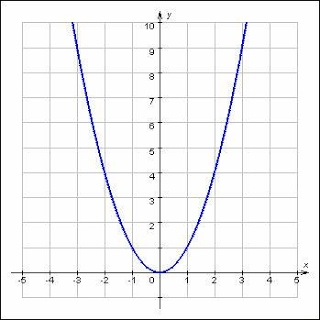
\includegraphics[width=0.5\textwidth]{img/par.jpg}
	\caption{Парабола}
\end{figure}

Общий вид параболы как мы знаем $y = ax^2 + bx + c$. Как мы разбирали в прошлой главе - это преобразования. Для определения конкретного преобразования используют прием - выделение полного квадрата:

\[
    x^2 + 2x - 5 = (x^2 +2x + 1) - 6 = (x + 1)^2 - 6
\]

И теперь видно, что это сдвиг элементарной функции $x^2$ по оси OX влево на 1 и сдвиг вниз по OY на 6.

Также для построения параболы удобно использовать формулу вершины параболы:

\[
    x_0 = -\frac{b}{2a} \text{, } y_0 = f(x_0)
\]

Аналитика функции относительно параметров a,b и c в $y = ax^2 + bx + c$:
\begin{itemize}
    \item Параметр c. Как и, например, в линейной функции b, это свободный член (без x), а значит что это в точности - пересечение графика с осью OY.
    \item Параметр a. как изучали в преобразованиях - это отражение относительно OX. Таким образом, положительное a - ветви вверх, отрицательное - ветви вниз.
    \item Параметр b. Данный параметр участвует в вершине параболы, а значит относительно знака b и a можно понять с какой стороны вершина параболы.
\end{itemize}

Также в построении графика можно использовать корни квадратного уравнения - это будут точки пересечения графика с осью OX.

\[
    x_{1,2} = \frac{-b \pm \sqrt{b^2 - 4ac}}{2a}
\]